\section{Results and Discussion}

We observed, as can be seen in Figure \ref{fig:results}., a small effect of
color on response time. All light conditions were lower than the non-light
conditions, with Green, Red, and Yellow lights having the lowest mean correct
response times (respectively, $0.649 \pm .017$, $0.666 \pm 0.020$, $0.656 \pm
0.018$, ms, $\pm$ SEM). With green having the lowest mean time. Green and Red
also had the fewest misses (TODO fig 2) with 1 each, compared to an average of
$3.0$ for all other colors, and $7$ for no light ($n=44$).


\vspace{2mm}
\begin{figure}[h!]
    \label{fig:results}
    \centering$
    \begin{array}{cc}
        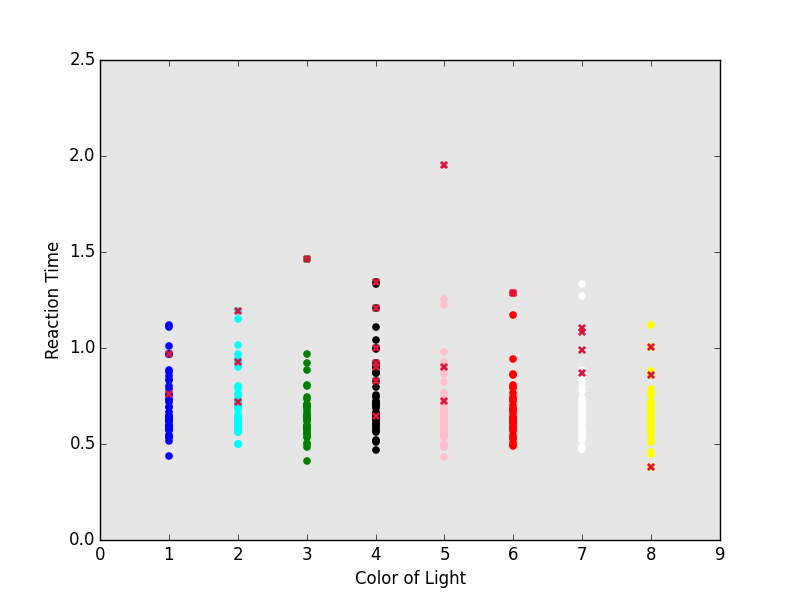
\includegraphics[width=0.5\textwidth]{figures/figure_1.png} &
        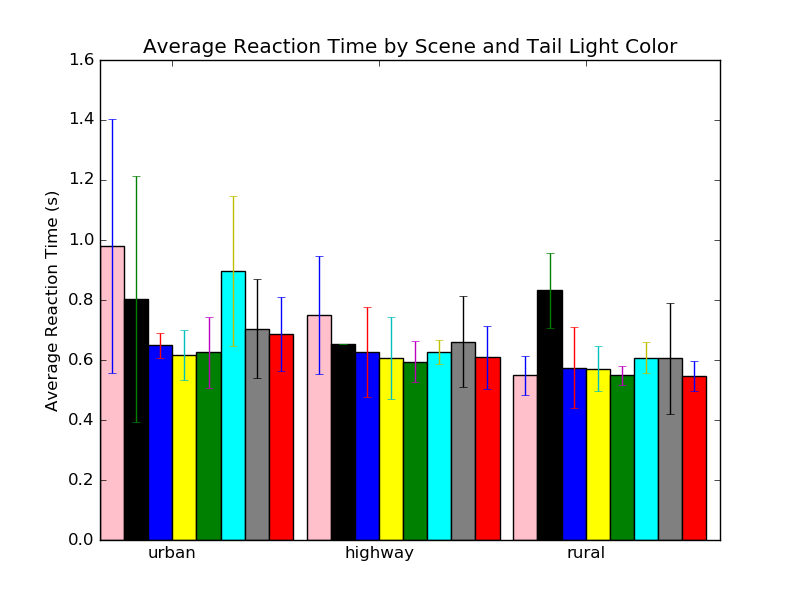
\includegraphics[width=0.5\textwidth]{figures/figure_2_alt.png}
    \end{array}$
    \caption{Results}
\end{figure}


%% Our original hypothesis was that as the target intensity value approached the
%% distractor intensity value, the search task would become ``serial search''.
%% Similarly, as the target-distractor intensity values diverged, the task would
%% become a trivial ``pop-out'' task.
%% 
%% Figure \ref{fig:results}. shows a plot of the average correct response time at
%% each of the 4 target intensity values. Each line represents the performance of
%% each of the three subjects. Looking at the results, it would have perhaps been
%% better to use more intensity values and less trials in order to gain a better
%% understanding on what possible functions could be fit to the phenomena.
%% However, qualitatively speaking, we can see a steep increase in response time
%% as the target intensity values approach that of the distractors, which
%% corroborates our hypothesis. We also note to our surprise that the performance
%% at opposite pairs of intensities, i.e. $0.95$ and $0.05$, are not necessarily
%% equivalent. Darker target intensities generally required less time to identify
%% than brighter target intensities for all three subjects.
%% 
%% 
%% It is also important to mention, that in conducting our experiment we observed
%% a distinct learning period, where despite more challenging target intensities,
%% subjects would become more adept at identifying the target the more trials they
%% would undergo. This was one of the greater challenges we faced when choosing
%% our final set of parameters.

